\subsection{Первое начало термодинамики. Работа. Теплота. Теплоемкость. Внутренняя энергия идеального газа}

\begin{definition}
    Внутренней энергией системы называется сумма кинетических энергий 
    хаотического движения всех молекул и потенциальных энергий 
    взаимодействия всех молекул друг с другом.
\end{definition}

\begin{definition}
    Вся внутренняя энергия идеального газа представляет собой 
кинетическую энергию теплового движения (потенциальная энергия 
взаимодействия молекул для идеального газа равна нулю). 
Внутренняя энергия одноатомного газа прямо пропорциональна его 
абсолютной температуре, массе газа, и обратно пропорциональна его 
молекулярному весу.

$$U = \bar E \cdot N = \frac{3}{2}kT\cdot \frac{m}{\mu}N_A = \frac{3}{2}\frac{m}{\mu}RT$$
\end{definition}

Для многоатомного газа: $U = \frac{i}{2}\frac{m}{\mu}RT$. (i - количество степеней свободы молекулы)

\begin{definition}
Процесс, при котором система возвращается в исходное положение, 
называется круговым, или циклом. 
Если система совершает круговой процесс (цикл), то
ее внутренняя энергия возвращается в исходное состояние. $\Delta U = 0$
\end{definition}

Изменение внутренней энергии системы в термодинамике может 
происходить двумя способами:
\begin{enumerate}
    \item за счет передачи системе тепла от окружающих ее тел; 
    \item за счет совершения этими телами работы над системой.
\end{enumerate}

\begin{definition}
    Работой в термодинамике называется процесс обмена энергией между 
    системой и окружающими ее телами вследствие изменения взаимного 
    расположения взаимодействующих тел.
    $A > 0$, если тело совершает работу над окружающими телами, и 
    $A < 0$, если тела совершают работу над системой.
\end{definition}

Работа при расширении газа

Газ в сосуде с поршнем, расширившись и сдвинув поршень, совершит работу: 
$$dA = Fdx = pSdx = pdV \implies A = \int\limits_{V_1}^{V_2} pdV$$

$V = const \implies A = 0$

$p = const \implies A = p(V_2-V_1)$

$pV=\frac{m}{\mu}RT \implies A = p\Delta V = \frac{m}{\mu}R\Delta T = \frac{m}{\mu} R(T_2-T_1)$

\begin{figure}[h]
    \centering
    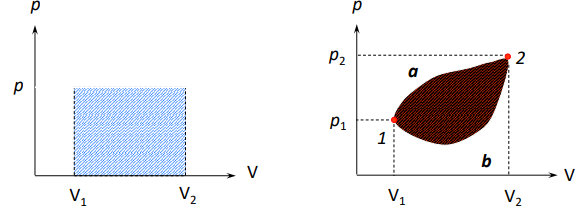
\includegraphics[width=0.5\linewidth]{imgs/q14i1.png}
    \caption{Графическое изображение работы}
\end{figure}

Работа зависит от пути перехода системы из состояния 1 в состояние 2.

Работа при круговом процессе (цикле):

Работа внешних сил по возвращению системы в исходное состояние 
может быть меньше работы, совершенной системой, т.е. в цикле иметь 
выигрыш работы.

\begin{definition}
    Теплоотдачей или теплообменом называется процесс обмена энергией 
    между системой и окружающими ее телами без совершения работы 
    только вследствие изменения внутренней энергии этих других тел.
\end{definition}

\begin{definition}
    Энергия, отдаваемая или получаемая системой в процессе теплообмена, 
    называется количеством тепла (теплотой). 
    $\Delta Q > 0$, если система получает тепло (нагревается), и 
    $\Delta Q < 0$, если система отдает тепло (охлаждается). 
\end{definition}

\begin{definition}
    Калория — внесистемная единица тепла, численно равная количеству 
    тепла, необходимого чтобы нагреть 1 г воды на 1 °С (от 19,5 °С до 20,5 °С). 

    1 кал = 4,18 Дж. 
\end{definition}

\begin{definition}
    Теплоемкостью тела называют скалярную физическую величину, 
    характеризующую связь между количеством сообщаемого системе тепла 
    и изменением ее температуры.

    Различают полную, удельную и молярную теплоемкость.
\end{definition}

\begin{definition}
    Полная теплоемкость тела численно равна количеству тепла, 
    необходимого для повышения температуры тела на 1 градус.

    $$C_{полн} = \frac{dQ}{dT} \implies dQ = C_{полн}dT$$
\end{definition}

\begin{definition}
    Удельная теплоемкость вещества численно равна количеству тепла, 
    необходимого для повышения температуры единицы массы вещества на 
    1 градус.

    $$c = \frac{dQ}{mdt} \implies dQ = cmdT$$
\end{definition}

\begin{definition}
    Молярная теплоемкость вещества численно равна количеству тепла, 
    необходимого для повышения температуры 1 моля вещества на 1 градус.

    $$C = \frac{dQ}{vdT} = \frac{dQ}{\frac{m}{\mu} dT} = \mu c$$
\end{definition}

\begin{remark}
    Теплоемкость газов зависит от характера процесса, при котором система 
получает тепло. Различают:
\begin{itemize}
    \item теплоемкость при постоянном давлении $C_p$
    \item теплоемкость при постоянном объеме $C_V$
\end{itemize}
\end{remark}

\begin{remark}
    Теплоемкость жидкостей и твердых тел

    Жидкие и твердые тела расширяются при нагревании незначительно, 
    поэтому их $С_p$ и $С_V$ практически не различаются.
\end{remark}

\begin{definition}
    Первым началом термодинамики называется закон сохранения энергии, 
распространенный на тепловые явления.
Изменение внутренней энергии системы при переходе ее из одного 
состояния в другое равно сумме работ внешних сил и количества теплоты, 
переданного системе.
\end{definition}

$$\Delta U = \Delta Q - A = \Delta Q + A'$$ 
$$\Delta Q = \Delta U + A$$

$A$ - работа внешних сил, $A'$ - работа газа

\begin{remark}
    Следствия из первого начала термодинамики:

    \begin{enumerate}
        \item Изолированная система
        
        Если система изолирована (теплота ей не передается и работа 
        над ней не совершается), то ее внутренняя энергия остается 
        неизменной (сохраняется). $\Delta Q = 0 \, , A = 0 \implies \Delta U = 0$
        
        \item Принцип эквивалентности тепла и работы
        
        При круговом процессе система не может совершать работу без 
        подвода тепла извне, или совершать работу большую, чем 
        подводимое к ней тепло. $\Delta U = 0 \implies A = \Delta Q$

        \item Вечный двигатель первого рода

        Если тепло к системе не подводится, то работа может быть 
        совершена только за счет убыли внутренней энергии $\Delta Q = 0 \implies A = -\Delta U$

        Невозможен вечный двигатель первого рода, т.е. устройство, 
        которое совершало бы работу без подвода энергии извне!

        \item Замкнутой системой тел называется такая система, которая не 
        обменивается ни энергией, ни веществом с окружающей средой.

        Внутренняя энергия замкнутой системы изменится не может! $\Delta U = \sum\limits_{i=1}^{n} \Delta U_i = 0$
    \end{enumerate}
\end{remark}

\begin{definition}
    Уравнение теплового баланса

    Алгебраическая сумма количеств теплоты, отданных и полученных в 
    замкнутой системе участвующими в теплообмене неподвижными телами, 
    равна нулю.

    $$\Delta Q = \sum\limits_{i=1}^{n} \Delta Q_i = 0 \implies \sum\limits_{i=1}^{n} m_i c_i (\Theta - t_i) = 0$$

    $\Theta$ - температура, установившаяся после наступления теплового равновесия.
\end{definition}


